\chapter{遗传算法的基础和应用}\label{chap:2}

\section{遗传算法的思想和简易流程}

\begin{figure}[!htbp]
    \centering
    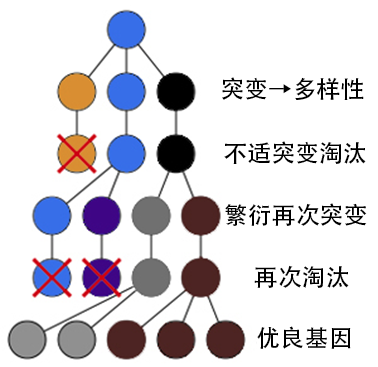
\includegraphics[width=0.6\textwidth]{Img/2-1.png}
    \caption{遗传算法的树状概念图,遗传算法通过在进化算法的基础上,引入类生物的算法操作,实现了更为直观有效的目标函数优化。生物种群的个体独立,天然具有并行计算的便利,据有现实的应用意义。}
    \label{fig:2-1}
\end{figure}
%%%%%%%%%%%%%%%%%%%%%%%%%%%%%%%%%%%%%%%%%%%%%%%%%%%%%%%%%%%%%%%%%%%%%%%%%%%%%%%%%%%%%%%%%%%%%%%%%%%%%%%%%%%%%%%%%%%%%%

遗传算法,是一种超启发式算法,属于进化算法中的一种。1960年由密歇根大学的计算机学家John H. Holland,在进化算法的基础上,受达尔文的进化论和自然选择过程的启发,引入基于生物的算法操作,如变异,杂交融合和自然选择等算法操作,用于产生、优化具有最高适应度的个体(匹配目标函数最优的解)。\cite{Genetic,2011yanshuhua}

在遗传算法中,通过一系列的候选个体的繁衍迭代,进化,选优,最终解决问题。

每个竞争的个体都有一系列的变量或属性(可以称为染色体),染色体可以进行变异或杂交变化。个体的染色体一般通过一系列0或1的二进制序列形式进行编码(如图2.2所示),而且编码长度相同,以便进行等位变量之间杂交处理。也可以采用其他数据类型的变量,通过类似的方法进行编码。

适应度(fitness)则是表征个体匹配目标函数之间的程度,越匹配目标函数,则适应度越高。不能匹配目标函数则适应度较低。

一旦基因表达的编码和适应度函数被定义后,遗传算法开始准备优化。初始化过程中,产生一系列的初始个体,并通过交叉,繁衍和自然选择等算法操作等操作改变个体的染色体,循环迭代,驱使个体的进化。

遗传算法的过程中,每一次的迭代称为一个代(generation)。在循环迭代的初始,一般从合适的初始种群出发,在每一代中,每个个体的基因进行修改,通过一定的数学方法,评估每个个体的适应度。从每个代的群体中,筛选适应性较好的个体,淘汰部分适应性较差的个体,从筛选出的个体中,通过一系列的生物算法操作操作,如交叉,变异等(如图2.2),新的个体产生伴随着父系的许多优异的特性。

生物算法操作的结果是子代的染色体对应的个体的平均的适应度会逐渐增加,因为上一代中较优适应度的染色体得以保留并繁育后代。同时一些中等适应度的染色体也得以保留,确保了基因池中的基因多样性,才能确保下一代个体可以通过组合形成更好的个体。

一般的,当达到了一定代数后,个体普遍达到较为满意的适应度,遗传算法则中止。

\begin{figure}[!htbp]
    \centering
    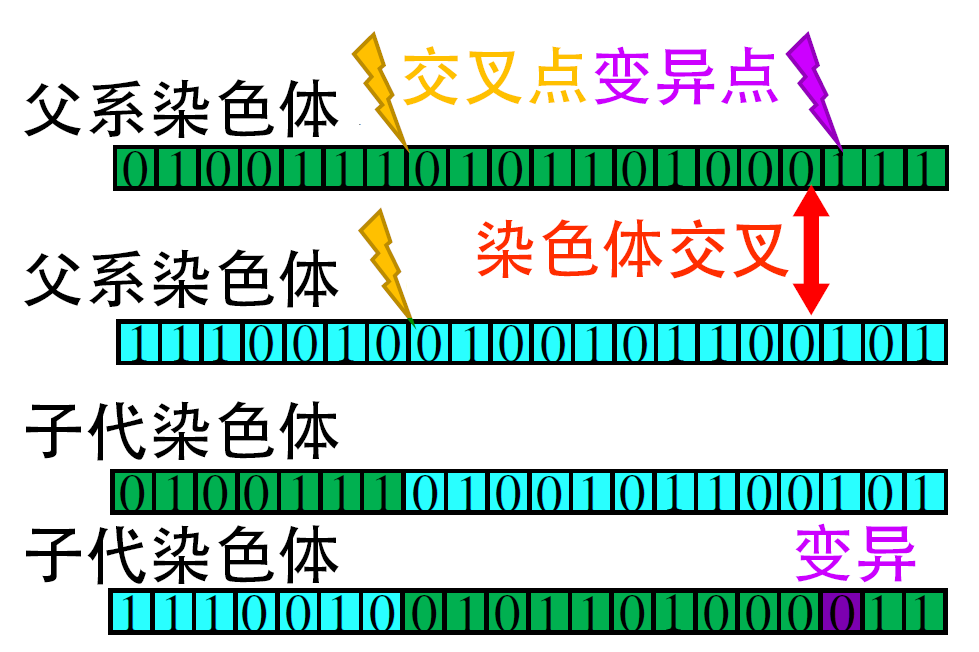
\includegraphics[width=0.8\textwidth]{Img/2-2.png}
    \caption{遗传算法中,从筛选出的适应度更高的个体中,通过染色体的交叉,形成一部分新的子代染色体。通过染色体上变量的突变,形成另一部分新的子代染色体。子代染色体通过重新组合,拥有了父系染色体的许多优异特性;也通过变异生成的新的染色体,丰富了多样性。}
    \label{fig:2-2}
\end{figure}
%%%%%%%%%%%%%%%%%%%%%%%%%%%%%%%%%%%%%%%%%%%%%%%%%%%%%%%%%%%%%%%%%%%%%%%%%%%%%%%%%%%%%%%%%%%%%%%%%%%%%%%%%%%%%%%%%%%%%%
\begin{figure}[!htbp]
    \centering
    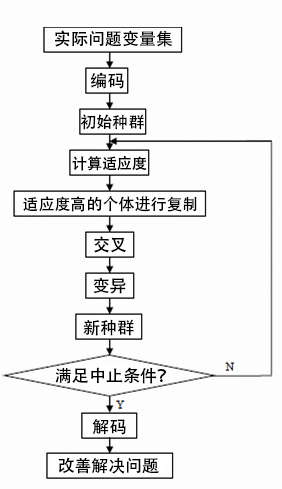
\includegraphics[width=0.6\textwidth]{Img/2-3.png}
    \caption{遗传算法的基础程序框图。程序的主体是个迭代的循环,像是生物繁衍的生生不息。通过个体筛选、交叉、变异等生物操作,实现了个体平均适应度的逐步提升,并最终改善、解决问题。}
    \label{fig:2-3}
\end{figure}
%%%%%%%%%%%%%%%%%%%%%%%%%%%%%%%%%%%%%%%%%%%%%%%%%%%%%%%%%%%%%%%%%%%%%%%%%%%%%%%%%%%%%%%%%%%%%%%%%%%%%%%%%%%%%%%%%%%%%%

一个基础的遗传算法的框架如图2.2所示,最开始从现实的问题的变量集开始,对待优化的变量进行编码,变成容易进行生物算法操作的染色体,数值优化。而后,从一个合理的初始种群开始。

对初始种群进行适应度计算,并将适应度高的个体进行筛选,再通过染色体的交叉,变异等类生物操作,实现了种群的繁衍和基因多样性的发展,完成了一个迭代循环。再通过第二次循环,计算新群体的适应度,交叉,变异等操作,当满足中止条件之后,达到最优化的个体编码。通过解码后的信息,改善并解决待优化的问题。

遗传算法的实现上,往往较为简单,可以通过2.2的程序框架,程序长度较短,自行纂写代码可以解决。也可以尝试调用开源的遗传算法工具包,实现严格、标准化的遗传算法程序实现。


\section{遗传算法的标准化工具包}

\begin{figure}[!htbp]
    \centering
    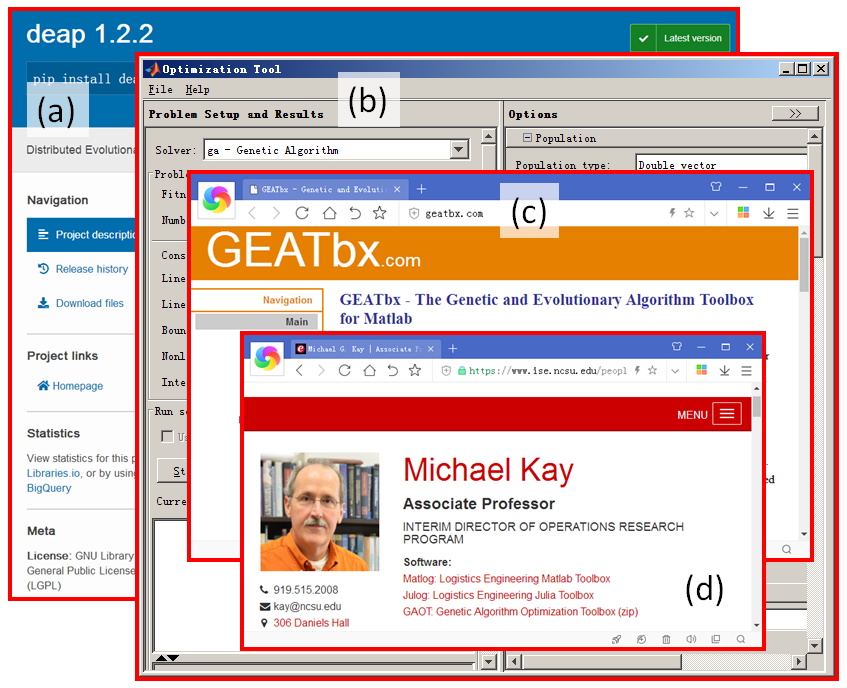
\includegraphics[width=1\textwidth]{Img/2-4.png}
    \caption{开源的遗传算法工具包。(a) 基于python的deap工具包。(b)MATLAB内置的optimtool工具包。(c)GEATbx工具包。(d) GAOT工具包。\cite{kay,geatbx,deap,Matlab}}
    \label{fig:2-4}
\end{figure}
%%%%%%%%%%%%%%%%%%%%%%%%%%%%%%%%%%%%%%%%%%%%%%%%%%%%%%%%%%%%%%%%%%%%%%%%%%%%%%%%%%%%%%%%%%%%%%%%%%%%%%%%%%%%%%%%%%%%%%

如图2.4所示,常用的开源遗传算法工具包有:

1、北卡罗来纳州立大学的Michael Kay助理教授的遗传算法工具包GAOT;\cite{kay}

2、德国伊尔姆瑙理工大学的Hartmut Pohlheim开发的GEATbx遗传算法和进化算法的MATLAB工具包;\cite{geatbx}

3、加拿大拉瓦尔大学的François-Michel De Rainville等人开发的基于python开源工具包deap;\cite{deap}

4、采用MATLAB内置的optimtool工具箱中的遗传算法优化功能。\cite{Matlab}



\section{遗传算法的应用案例和启发}
\begin{figure}[!htbp]
    \centering
    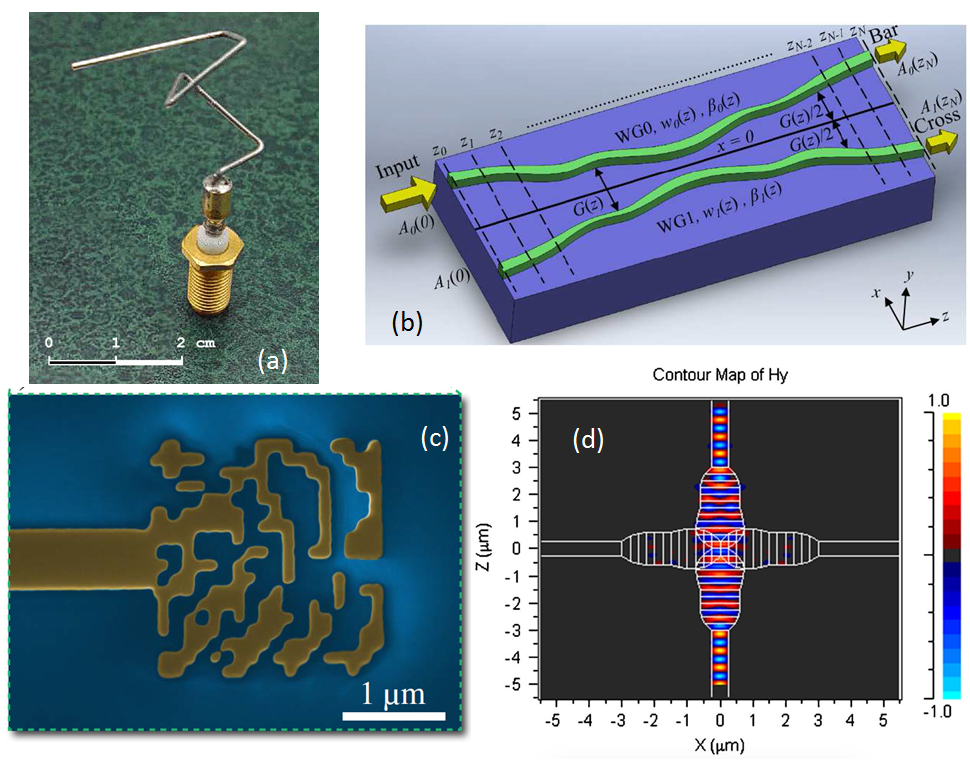
\includegraphics[width=1\textwidth]{Img/2-5.png}
    \caption{遗传算法优化器件的案例。}
    \label{fig:2-5}
\end{figure}
%%%%%%%%%%%%%%%%%%%%%%%%%%%%%%%%%%%%%%%%%%%%%%%%%%%%%%%%%%%%%%%%%%%%%%%%%%%%%%%%%%%%%%%%%%%%%%%%%%%%%%%%%%%%%%%%%%%%%%



有了遗传算法,们可以方便地引入到各种各样的光学器件的优化设计中,如图2.4所示。

图2.4a为遗传算法在电磁波优化中最为经典的案例之一,加利福尼亚大学圣克鲁兹分校的Gregory S. Hornby等人,在美国国家航空航天局Space Technology 5(NASA ST5)项目中采用的射频天线,该天线为通过遗传算法优化的折线结构,与以往规整的天线结构相比格外另类,然而这种特殊折线结构可以实现更好的微波波束辐射。\cite{Hornby2010Automated}

图2.4b为国立台湾大学的Po-Han Fu等人,通过耦合模理论(coupled-mode theory)结合遗传算法优化的方向耦合器,可以实现任意分光比的光功率分束。\cite{Fu2016Broadband}

图2.4c为香港中文大学的Zejie Yu等人,通过遗传算法优化的数字超材料波导反射器,在2×2$\mu$m$^2$的硅超材料结构上,实现了200nm宽光的谱的高反射效率。\cite{Zejie2017Genetically}

图2.4d为西班牙瓦伦西亚理工大学的Pablo Sanchis等人,通过遗传算法优化光交叉的波导截面宽度,在6×6$\mu$m$^2$的器件尺寸下,实现-0.2dB低插入损耗和-35dB的低串扰的紧凑光交叉耦合器。\cite{Pablo2009Highly}

通过上述案例,足以可见遗传算法在光学器件优化中的广泛作用和潜力。\cite{Sanchis2004Integrated,Jyun2014Genetic}


